\lesson{}{Machine Learning}

\section{Deep Neural Networks}
\subsection{Multi-Layer Perceptron}
\FloatBarrier
\begin{figure}[ht]
   \centering
   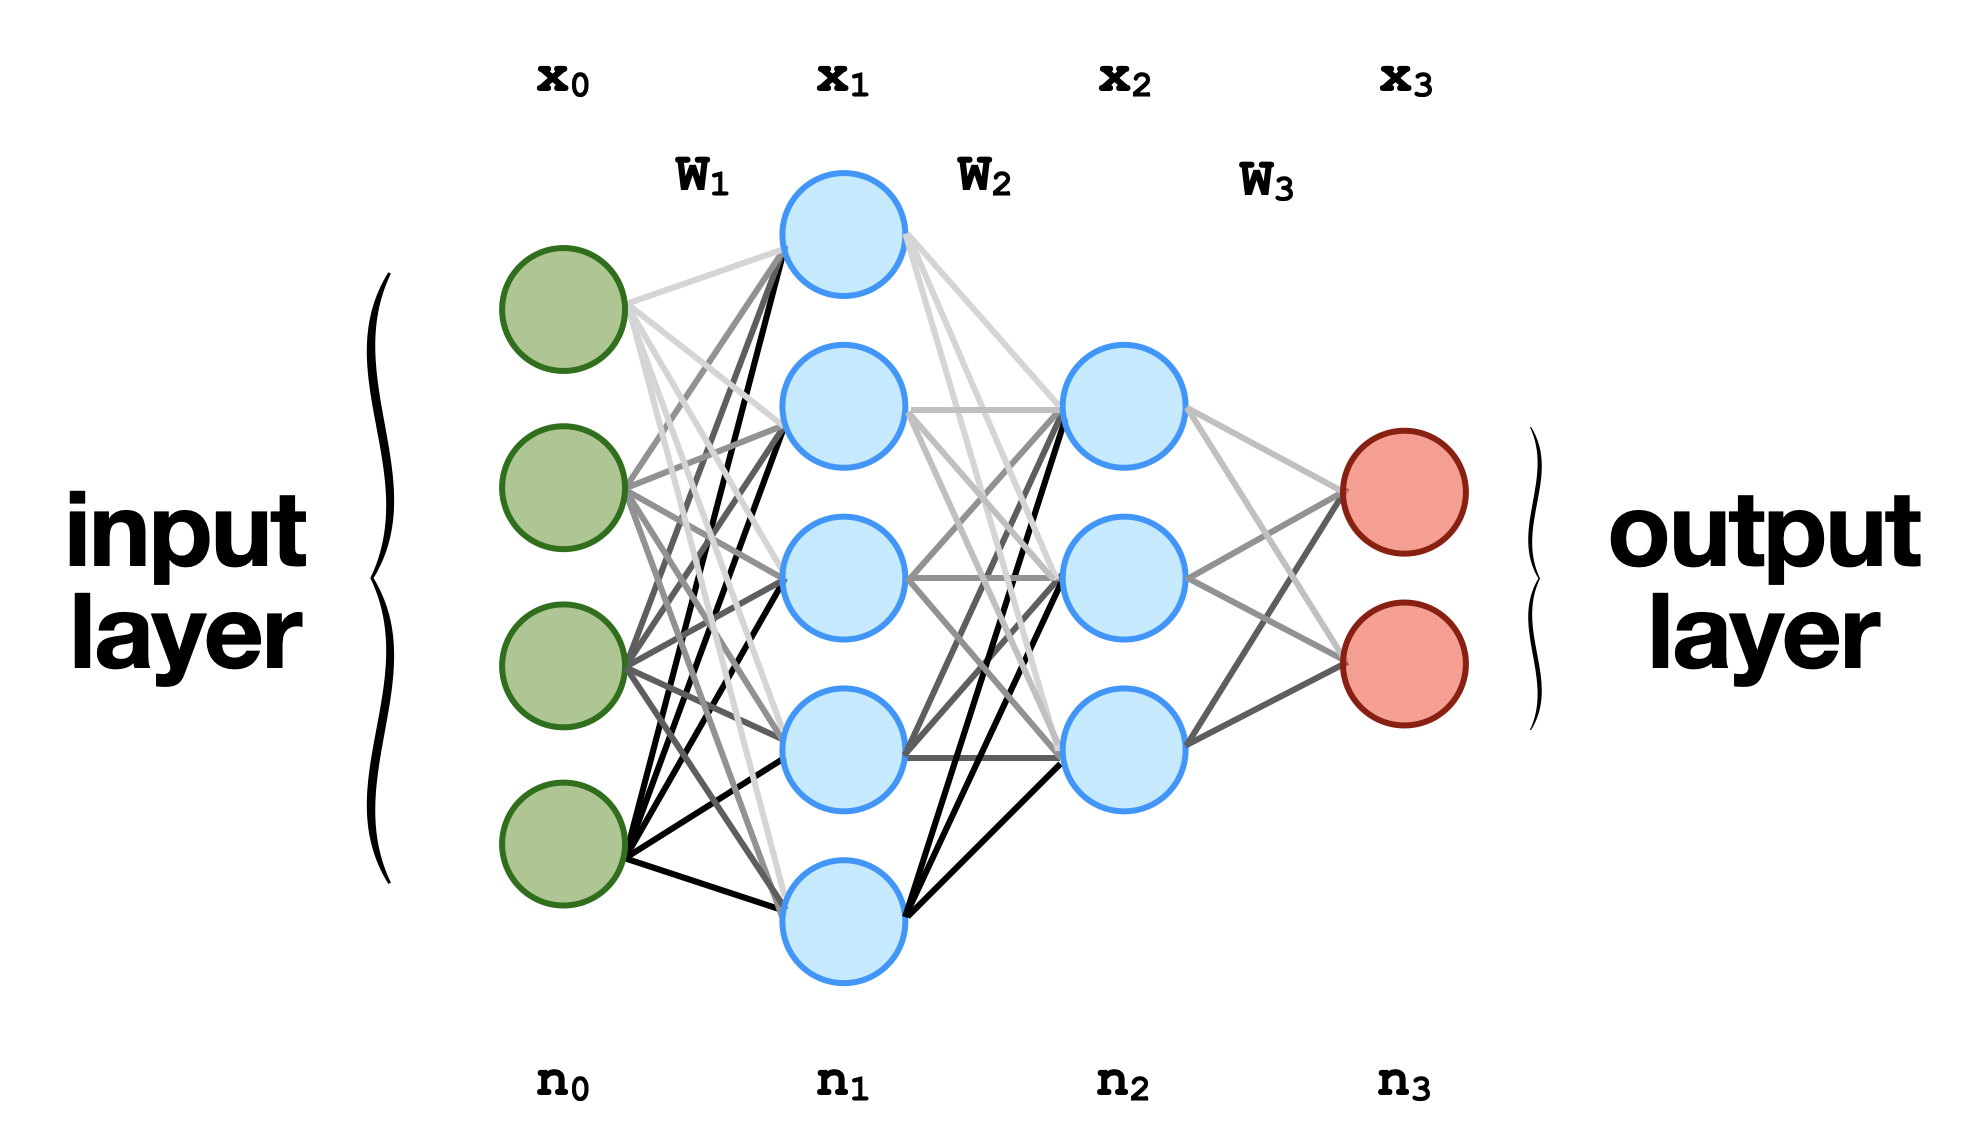
\includegraphics[width=0.75\textwidth]{figures/mlp.png}
   \caption{A typical visual representation of fully-connected 4-layer neural network or multi-layer perception (MLP) where $\boldsymbol{x}_i$ is input vector to the next layer, $\boldsymbol{W}_i$ are te matrix weights, and $n_i$ are the number of neurons in a layer. }
   \label{fig:mlp}
\end{figure}
\FloatBarrier

Neural networks are a subset of machine learning algorithms that are designed to model the behavior of the human brain. They are composed of interconnected nodes or neurons, which are organized into layers and process information in a parallel and distributed manner. Neural networks have gained significant attention in recent years due to their ability to solve complex problems in various domains, including image and speech recognition, natural language processing, and predictive analytics. One of the key strengths of neural networks is their ability to approximate any function to arbitrary accuracy, given a sufficiently large number of neurons in the hidden layers. This property, known as universal approximation, has made neural networks an essential tool for data scientists and researchers seeking to develop intelligent systems capable of learning and adapting to changing environments. In this background section, we will provide a comprehensive overview of the fundamentals of neural networks, including their architecture, training algorithms, and applications.



Multi-layer perceptions (MLPs) are a class of feed-forward neural networks that consist of one or more hidden layers of fully connected neurons (see \Cref{fig:mlp}). In an MLP, each neuron receives inputs from all the neurons in the previous layer and computes a weighted sum of these inputs with additional bias term $b$. The weighted sum is then passed through an activation function, which introduces non-linearity into the model. The most commonly used activation functions include \texttt{sigmoid}, \texttt{ReLU}, and \texttt{tanh}. The output of each neuron is then passed on to the neurons in the next layer until the output layer is reached, which produces the final output of the network. This sequence of operations is typically referred to as the \textit{forward pass}. The neural network \textit{learns} by iteratively updating itself using optimization methods that minimizes the error between output of the neural network and the output from the training data, also known as the \textit{backward pass} or \textit{backward propagation}. 

\vspace{0.5cm}
\noindent \textit{Forward Pass} 
\vspace{0.25cm}

The computations performed by the neurons in an MLP can be mathematically represented as matrix-vector multiplication, where the weights of each neuron in a layer are represented as a row in a weight matrix. Consider the MLP represented in \Cref{fig:mlp}. The first layer contains four input nodes, which can be represented as an input vector $\boldsymbol{x}_0 \in \mathcal{R}^{n_0 + 1}$. The additional dimension is a place holder for the bias term $b$. The non-linear mapping between each layer begins with a linear matrix-vector operation between the preceding layer and its corresponding weight matrix $W_1 \in \mathcal{R}^{n_1 \times n_0 + 1}$. The output of this matrix is passed element-wise through a non-linear activation function of the user's choice. The output of this operation has a dimension equal to the size of the subsequent layer. Explicitly, this operation is

\begin{equation}
    \phi\big(\boldsymbol{W}_1 \boldsymbol{x}_0 \big) = 
    \phi\bigg(
    \begin{bmatrix}
W_{0,0}^{1} & W_{0,1}^{1} & W_{0,2}^{1} & W_{0,3}^{1} & b_0\\
W_{1,0}^{1} & W_{1,1}^{1} & W_{1,2}^{1} & W_{1,3}^{1} & b_1\\
W_{2,0}^{1} & W_{2,1}^{1} & W_{2,2}^{1} & W_{2,3}^{1} & b_2\\
W_{3,0}^{1} & W_{3,1}^{1} & W_{3,2}^{1} & W_{3,3}^{1} & b_3\\
W_{4,0}^{1} & W_{4,1}^{1} & W_{4,2}^{1} & W_{4,3}^{1} & b_4\\
% W_{5,0}^{1} & W_{5,1}^{1} & W_{5,2}^{1} & W_{5,3}^{1} & b_5\\
\end{bmatrix}
\begin{bmatrix}
    x_0^{0} \\
    x_1^{0} \\
    x_2^{0} \\
    x_3^{0} \\
    1
\end{bmatrix} 
\bigg)
= \boldsymbol{x}_1 
\end{equation}

where $W_{i,j}^{1}$ represents the element in the $(i+1)$-th row and $(j+1)$-th column of the weight matrix $W_1$, using zero-indexing, the superscript $1$ indicates that $\boldsymbol{W}$ is weight matrix mapping to the first layer, and $\phi$ represents the activation function of choice. 

Iterating this non-linear mapping procedure through each subsequent layer in \Cref{fig:mlp} yields the following result 

\begin{equation}
    \psi\bigg(\boldsymbol{W}_3 
    \underbrace{\phi\big(\boldsymbol{W}_2 
    \underbrace{\phi(W_1 \boldsymbol{x}_0)}_{\boldsymbol{x}_1}
    \big)}_{\boldsymbol{x}_2}\bigg) = \boldsymbol{x}_3. 
\end{equation}

where the outer activation function $\psi$ is the soft max function used to produce a probability distribution over the possible output classes.


\vspace{0.5cm}
\noindent \textit{Backward Pass}
\vspace{0.25cm}

When training a model, inputs from a training data set are passed through a neural network following the matrix-vector multiplications provided above and the error between the outputs of the neural network and the training data can mathematically defined as the norm of the differences between both outputs: 

\begin{equation}
    \mathcal{L} = \frac{1}{2}|| \boldsymbol{x}_3 - \boldsymbol{t}||_2
\end{equation}

where $\boldsymbol{x}_3$ is the output of the neural network, $\boldsymbol{t}$ is the ground truth from the training data, and $\mathcal{L}$ is the \textit{loss}. Although there are a variety of optimization methods  (more methods are discussed in later in this chapter) for determining the weights, the widely accepted approach is a first order gradient descent method \cite{kochenderfer2019algorithms}: 

\begin{equation}
    \boldsymbol{W}^{n+1}_i = \underbrace{\boldsymbol{W}^{n}_i}_{\in \mathcal{R}^{n_i \times n_{i-1} + 1}} - \underbrace{\alpha  \nabla_{\boldsymbol{W}_i} \mathcal{L}}_{\in \mathcal{R}^{n_i \times n_{i-1} + 1}}
\end{equation}

where $i = 1, \dots, m$ represents the total number of transitions between layers. For the four layer network in \Cref{fig:mlp}, there are three transitions meaning back propagation of this network will required differentiating $\mathcal{L}$ with respect to three weight matrices, $\boldsymbol{W}_1$, $\boldsymbol{W}_2$, and $\boldsymbol{W}_3$. 

\vspace{0.5cm}
\noindent\textit{Back propagation of a four-layer fully connected neural network}
\vspace{0.25cm}

The loss function we want to minimize is the $L_2$ norm of the difference between the output of the network and the training data: 

\begin{equation}
    \mathcal{L} = \frac{1}{2}||\boldsymbol{x}_3 - \boldsymbol{t}||_2^2 = \frac{1}{2} (\boldsymbol{x}_3 - \boldsymbol{t})^\top (\boldsymbol{x}_3 - \boldsymbol{t})
\end{equation}

where the explicit equation for the neural network is: 

\begin{equation}
    \boldsymbol{x}_3 = \psi\Bigg(\boldsymbol{W}_3 \phi\bigg(\boldsymbol{W}_2 \phi\big(\boldsymbol{W}_1 \boldsymbol{x}_0\big)\bigg)\Bigg). 
\end{equation}

To update the next guess matrix for $\boldsymbol{W}_i$, we need to compute the gradients $\nabla \mathcal{L} = [\frac{\partial \mathcal{L}}{\partial \boldsymbol{W}_1}, \frac{\partial \mathcal{L}}{\partial \boldsymbol{W}_2}, \frac{\partial \mathcal{L}}{\partial \boldsymbol{W}_3}]$. It is important to note that since we are dealing partial derivatives with respect to matrices and vectors, the gradient of the loss function is actually a vector of matrices. The derivatives are obtained by using the chain rule: 

\begin{equation}
    \frac{\partial \mathcal{L}}{\partial \boldsymbol{W}_1} = \frac{\partial \mathcal{L}}{\partial \boldsymbol{x}_3} \circ \frac{\partial \boldsymbol{x}_3}{\partial \boldsymbol{x}_2} \circ \frac{\partial \boldsymbol{x}_2}{\partial \boldsymbol{x}_1} \circ \frac{\partial \boldsymbol{x}_1}{\partial \boldsymbol{W_1}} \circ \boldsymbol{x}_0^\top
\end{equation}
 
 


\noindent An explicit computation of backpropagation is shown below. 

\begin{align}
    \frac{\partial \mathcal{L}}{\partial \boldsymbol{W}_1} &= (\boldsymbol{x}_3 - \boldsymbol{t}) \circ \psi^{\prime} (\boldsymbol{W}_3 \boldsymbol{x}_2) \circ \boldsymbol{W}_3 \phi^\prime (\boldsymbol{W}_2 \boldsymbol{x}_1) \circ \boldsymbol{W}_2 \phi^\prime(\boldsymbol{W}_1\boldsymbol{x}_0) \circ \boldsymbol{x}_0^\top \\
    \frac{\partial \mathcal{L}}{\partial \boldsymbol{W}_1} &= (\boldsymbol{x}_3 - \boldsymbol{t}) \circ \psi^\prime(\boldsymbol{W}_3 \boldsymbol{x}_2) \circ \boldsymbol{W}_3 \phi^\prime(\boldsymbol{W}_2 \boldsymbol{x}_1) \boldsymbol{x}_1^\top \\
    \frac{\partial \mathcal{L}}{\partial \boldsymbol{W}_3} &= \underbrace{\underbrace{(\boldsymbol{x}_3 - \boldsymbol{t})}_{\in \mathcal{R}^{n_3}} \circ \underbrace{\psi^\prime(\boldsymbol{W}_3 \boldsymbol{x}_2)}_{\in \mathcal{R}^{n_3}} }_{\begin{bmatrix} v_1 \\ v_2\end{bmatrix}} \underbrace{\underbrace{\boldsymbol{x}_2^\top}_{\in \mathcal{R}^{1 \times n_2 + 1}} }_{\begin{bmatrix} x_2^{(1)} & x_2^{(2)} & x_2^{(3)} & 1 \end{bmatrix}}
\end{align}

where $\circ$ is the Hadamard product, and the final operation for each partial derivative is an outer product. 
    

Inference from neural networks refers to the process of using a trained model to make predictions or decisions on new input data. During inference, the input data is passed through the network, which performs the sequential matrix-vector operations with the weights $\boldsymbol{W}_i$ obtained from training on the input to generate an output. The output is then used to make a prediction or decision based on the task the network was trained to perform, such as image classification or natural language processing. Inference is an important step in using neural networks for real-world applications, as it allows the model to be applied to new data and provide useful insights or actions.

\subsection{Automatic Differentiation}


In machine learning, the successful training of complex neural networks and mathematical models hinges upon the seamless interplay between two fundamental processes: optimization, which fine-tunes model parameters to minimize or maximize a specific objective, and backpropagation, which efficiently computes gradients essential for guiding the optimization process. Central to the efficacy of these processes are automatic differentiation tools, which provide a systematic and computationally efficient way to compute gradients of complex functions. Automatic differentiation techniques have emerged as a cornerstone technology, enabling the training of deep learning architectures and other optimization-driven algorithms. This methods-focused exposition delves into the landscape of automatic differentiation, elucidating its pivotal role in the domains of optimization and backpropagation. We explore the underlying principles of automatic differentiation, encompassing both forward and reverse modes, while highlighting prominent automatic differentiation frameworks and their integration within optimization algorithms. By elucidating the symbiotic relationship between automatic differentiation, optimization, and backpropagation, this section aims to equip practitioners with a comprehensive understanding of the techniques that underpin the training of modern machine learning models. 

As indicated in the preceding section, deep learning is predicated on the successive matrix-vector operations followed by a non-linear activation function. Back-propagation requires differentiating through the entire network and requires a computational approach to keep track of an arbitrary number of mathematical operations. The fundamental representation in automatic differentiation is the computation graph which serves as a structured visualization of the transformations and computations that occur within a model during its forward pass. 

By analyzing the chain of operations encoded within the computational graph, automatic differentiation enables the extraction of derivatives, facilitating efficient gradient computation for optimization algorithms like stochastic gradient descent. This dynamic interplay between computational graphs and automatic differentiation forms the foundation upon which modern optimization-driven machine learning thrives, engendering the ability to train intricate models while efficiently updating their parameters through gradient-based techniques.

\newpage